\quad \textbf{Пример пары заданий одного типа, на основе которых создан следующий шаблон. } 

\begin{figure}[h]
		\centering
		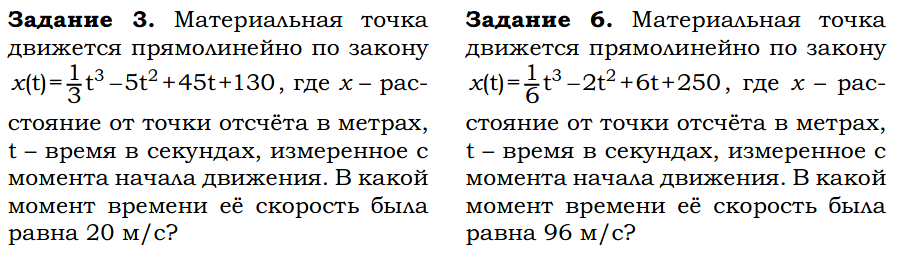
\includegraphics[width=1\linewidth]{VM/Пример.png}
\label{ris:image}
\end{figure}

\quad Первая часть шаблона выглядит следующим образом:
	\begin{figure}[h]
		\centering
		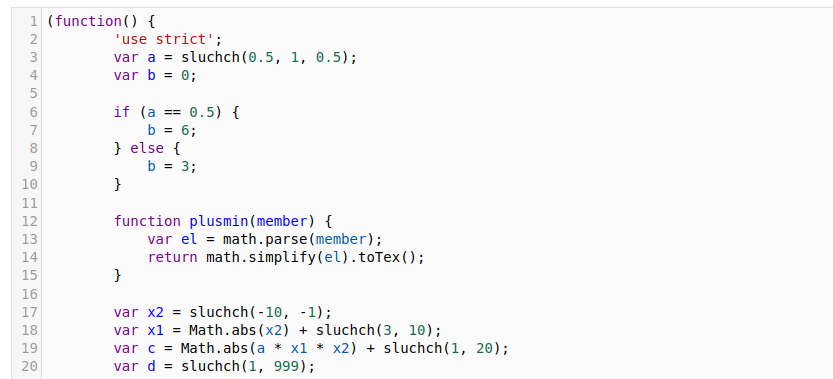
\includegraphics[width=1.2\linewidth]{VM/1.1.png}
	\end{figure}

\quad Здесь объявляются переменные таким образом, чтобы генерируемые значения,  максимально соотносились с исходной задачей.
\\ В этой части также используются специальные встроенные функции, такие как:
\\ \textbf{sluchch(a, b)} – функция случайным образом возвращает число из диапазона от «a» до «b». Если функции добавить третье число sluchch(a, b, с), то она будет возвращать случайно число уже с шагом «с».
\\ \textbf{Math.abs(a)} – функция возвращает модуль числа «a».
\\ \textbf{function plusmin(member)} – функция принимает аргумент, содержащий в себе пример, наподобие: «1*a+-b». И возвращает его упрощённый вариант: «a-b».
\\
\quad Вторая часть выглядит следующим образом:
	\begin{figure}[h]
		\centering
		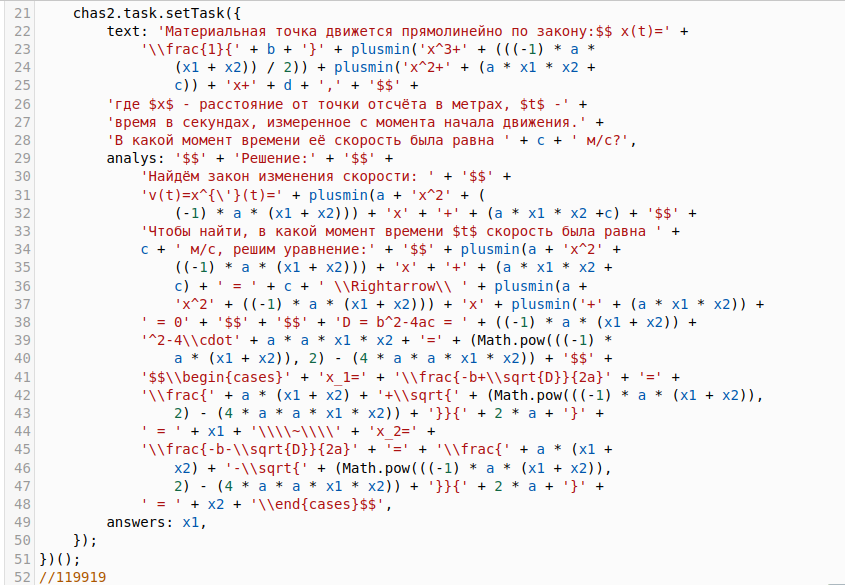
\includegraphics[width=0.85\linewidth]{VM/2.2.png}
	\end{figure}

\quad Вторая часть программы делится на несколько составных частей:
\\ условие задачи, записанное после «text:»
\\ решение, записанное после «analys:».
\\ ответ, записанный после «»answer.
\\ \quad В этом шаблоне мы вводим переменные, генерирующие случайные значения, которые используем для составления ответа. И на основе ответа мы уже составляем саму задачу и её решение.
\\ \quad  В этой части также используются некоторый команды latex, например:
\\ \textbf{\textbackslash frac} – функция выводящая дробь на экран.
\\ \textbf{\textbackslash Rightarrow} – функция выводящая двойную стрелку вправо
\\ \textbf{\textbackslash begin\{cases\}} и \textbf{\textbackslash end\{cases\}} – окружение, выводящая фигурную скобку на экран. 
\\
\\
\textbf{Задачи из ЕГЭ по математике базового уровня тип №16}
	\begin{figure}[h]
		\centering
		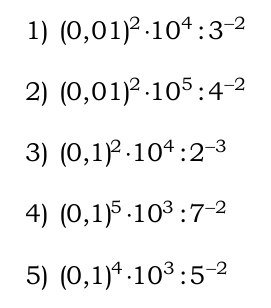
\includegraphics[width=0.3\linewidth]{VM/t16.1.png}
		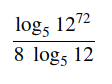
\includegraphics[width=0.15\linewidth]{VM/t16.3.png}
	\end{figure}
	
\quad \textbf{Шаблоны задач}
\\
\begin{figure}[h]
		\centering
		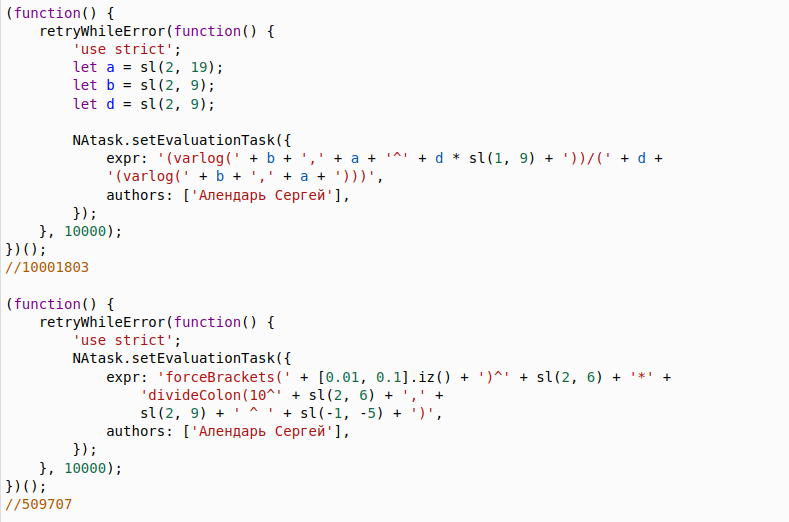
\includegraphics[width=1\linewidth]{VM/t16k.png}
	\end{figure}
	
\quad Отличительной особенностью этих шаблонов от предыдущего, является другая библиотека - setEvaluationTask. Помимо самой генерации задачи, на основе переменных их первой части, она так же сама решает сгенерированный пример, и проверяет его ответ. 
\\ \quad Если ответ не является удовлетворительным, а именно таким, что пользователь просто не сможет ввести его на клавиатуре (Ответ представляет из себя бесконечную десятичную дробь, ну или просто очень длинную), то программа, отслеживает эту ошибку с помощью цикла "retryWhileError" и предпринимает ещё попытку составить задание с цельным ответом. Количество таких попыток указано внизу кода программы. Если за установленное число попыток, программа так и не получит правильно сгенерированную задачу, то она выведет сообщение об ошибке.
\\ \quad В этих шаблонах тоже используются некотрые свои специальные встроенные функции, например:
\\ \textbf{varlog} - отвечает за отображение логарифма на экране.
\\ \quad Также эта библиотека способна сама убирать некоторые скобки, если они не влияют на решение задания, или сама выполнть арифметическую операцию. Но в некотрых случаях, это не является необходимостью. Чтобы программа не высчитывала сама, то что стоит оставить, используются следующие команды:
\\ \textbf{forceBrackets} - для сохранение скобок.
\\ \textbf{divideColon} - для вывода знака деления ":".

\quad \textbf{Сгенерированные по шаблонам задания}

\begin{figure}[h]
		\centering
		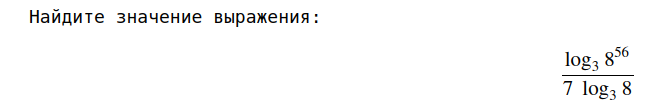
\includegraphics[width=0.6\linewidth]{VM/log1.png}
		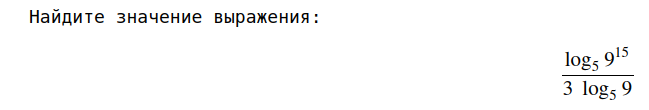
\includegraphics[width=0.6\linewidth]{VM/log2.png}
		\end{figure}
		\begin{figure}[h]
		\centering
		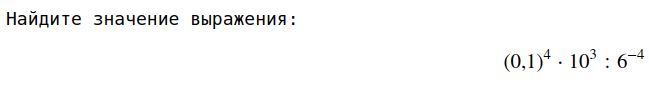
\includegraphics[width=0.6\linewidth]{VM/skob1.png}
		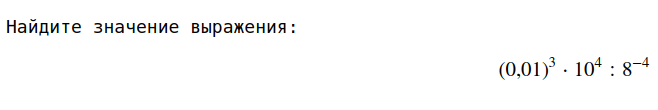
\includegraphics[width=0.6\linewidth]{VM/skob2.png}
\end{figure}
\quad \textbf{Задача №77381 тип №6}

\begin{figure}[h]
	\centering
	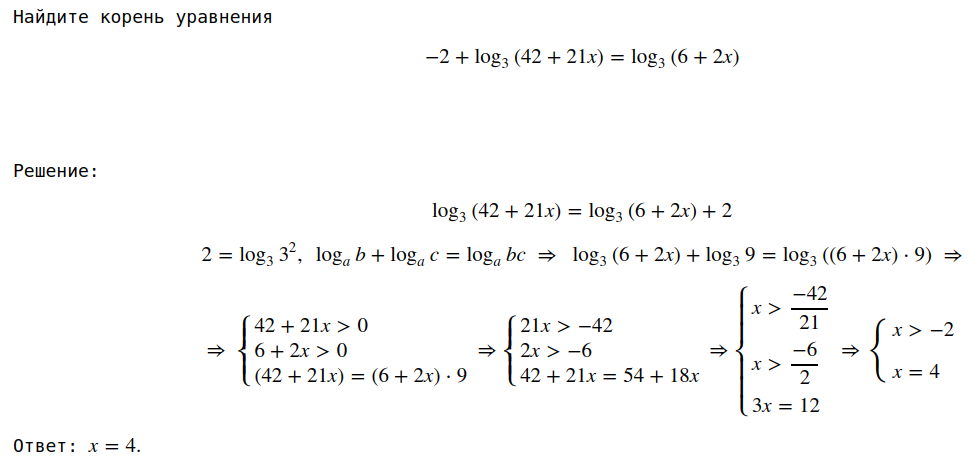
\includegraphics[width=0.9\linewidth]{VM/log.png}
\end{figure}

\newpage

\quad Первая часть шаблона
	
\begin{figure}[h]
		\centering
		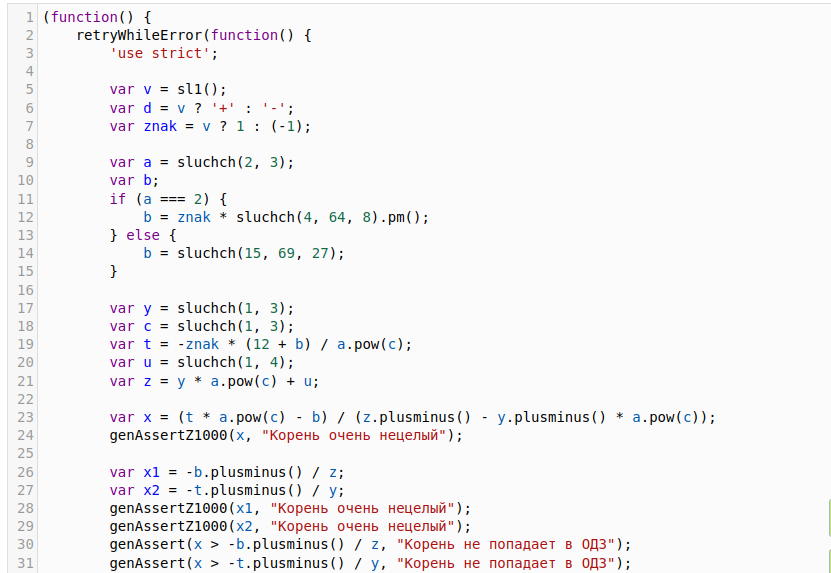
\includegraphics[width=0.9\linewidth]{VM/1log.png}
		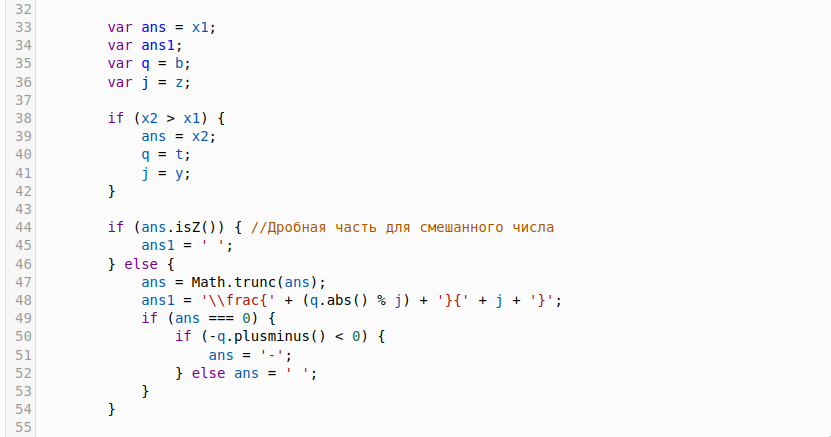
\includegraphics[width=0.9\linewidth]{VM/2log.png}
\end{figure}

\newpage

\quad Вторая часть шаблона

\begin{figure}[h]
		\centering
		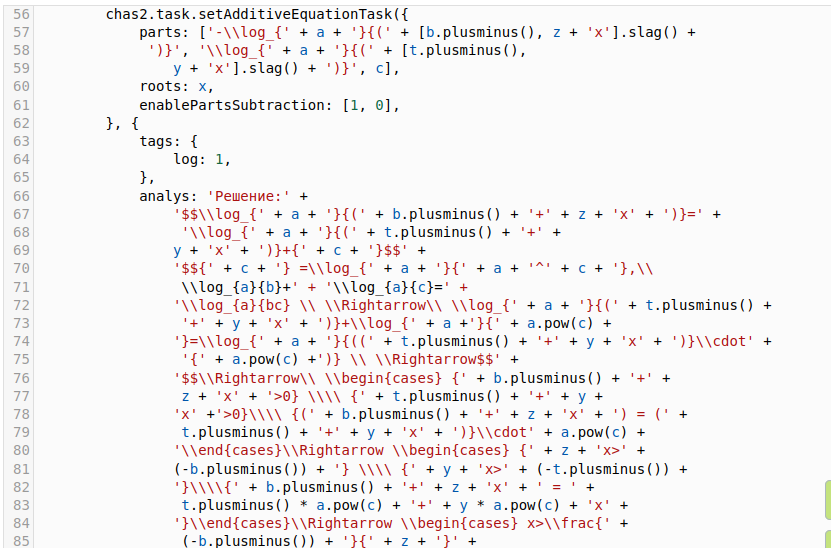
\includegraphics[width=0.96\linewidth]{VM/3log.png}
		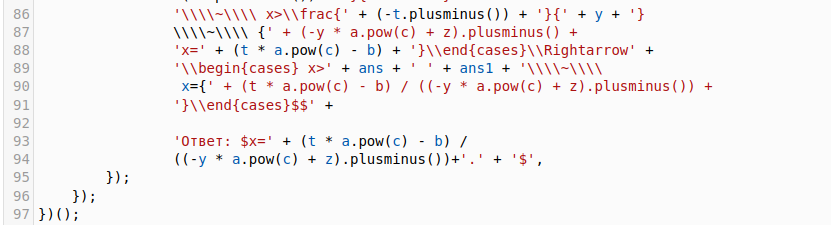
\includegraphics[width=0.96\linewidth]{VM/4log.png}
\end{figure}

\quad \textbf{Задачи, сгенерированные по шаблонам, использующим код 
\\ арифметической прогрессии.}
	\begin{figure}[h]
		\centering
		
\includegraphics[width=1\linewidth]{VM/1 (1).png}
		
\includegraphics[width=1\linewidth]{VM/2 (1).png}
		
\includegraphics[width=1\linewidth]{VM/3 (1).png}
	\end{figure}
	
\newpage

\quad \textbf{Код арифметической прогрессии}

	\begin{figure}[h]
		\centering
		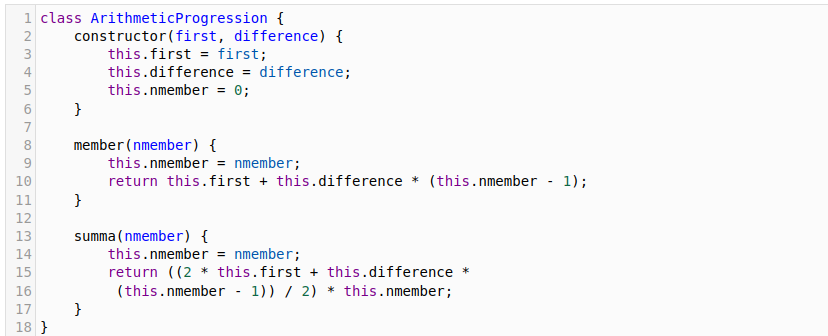
\includegraphics[width=1.1\linewidth]{VM/3b.png}
		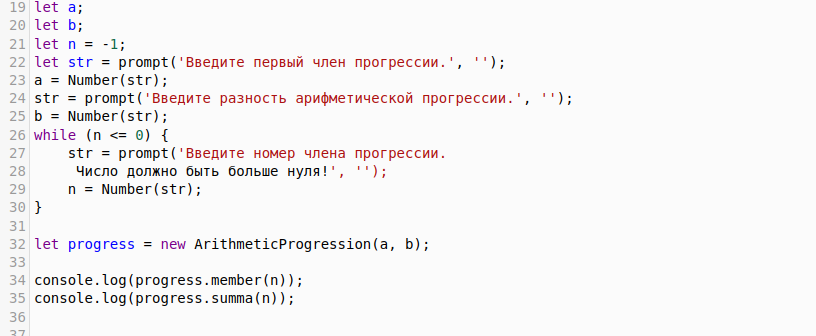
\includegraphics[width=1.1\linewidth]{VM/3c.png}
	\end{figure}

\quad \textbf{Задачи, сгенерированные по шаблонам, использующим код 
\\геометрической прогрессии.}

	\begin{figure}[h]
		\centering
		
\includegraphics[width=1\linewidth]{VM/4 (1).png}
		
\includegraphics[width=1\linewidth]{VM/5 (1).png}
	\end{figure}
	
\quad \textbf{Код геометрической прогрессии}

\newpage

\begin{figure}[h]
		\centering
		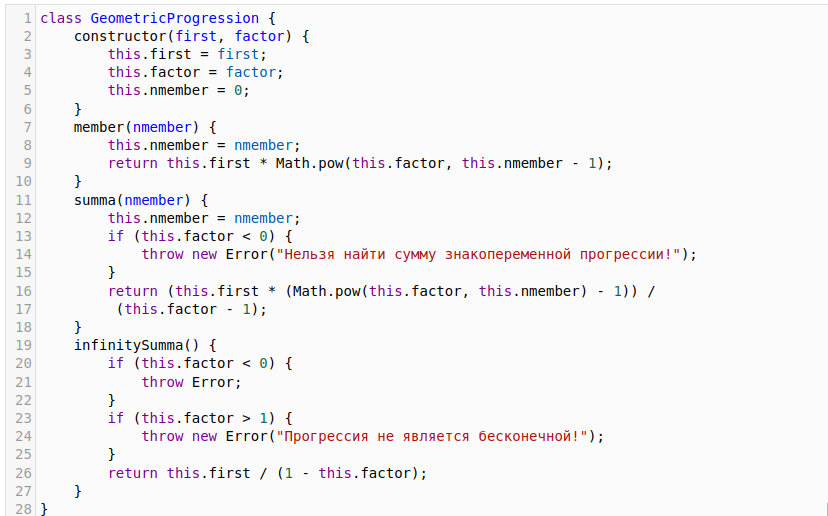
\includegraphics[width=0.9\linewidth]{VM/4b.png}
		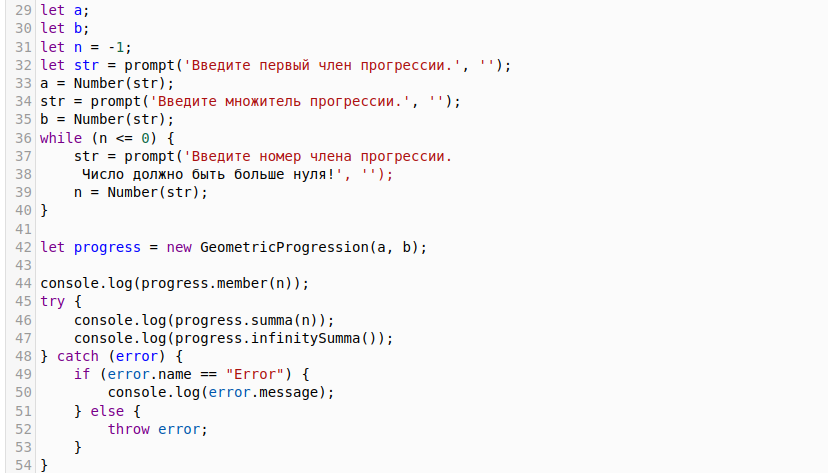
\includegraphics[width=0.9\linewidth]{VM/4c.png}
	\end{figure}
	
\newpage

\quad \textbf{Тригонометрическая задача №77492}

	\begin{figure}[h]
		\centering
		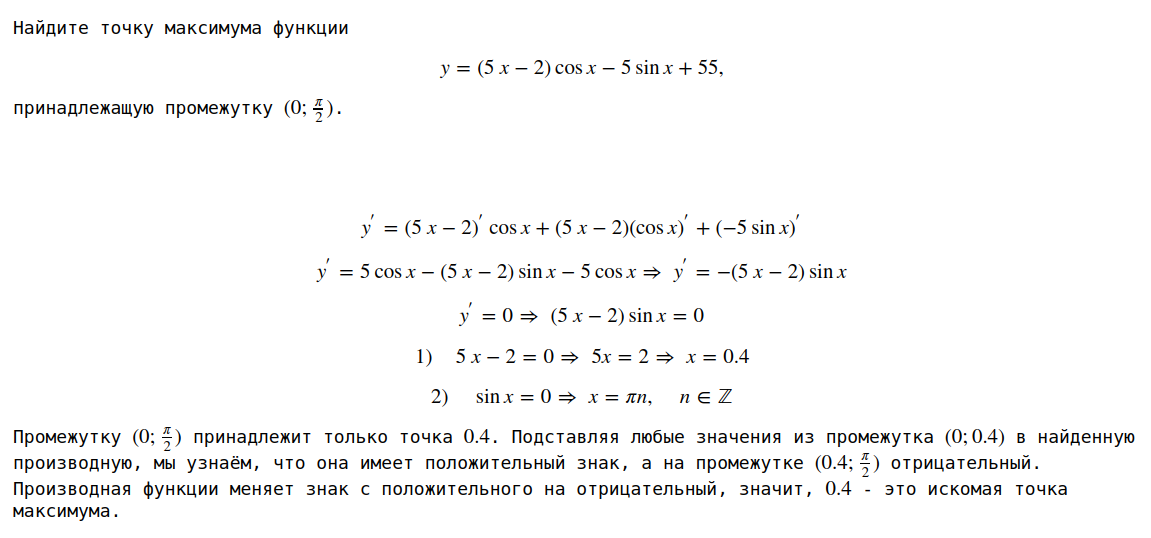
\includegraphics[width=1\linewidth]{VM/7 (1).png}
	\end{figure}

\quad \textbf{Код для задачи №77492}

\begin{figure}[h]
		\centering
		\includegraphics[width=1\linewidth]{VM/7б.png}
\end{figure}
			
\begin{figure}[h]
		\centering
		\includegraphics[width=1\linewidth]{VM/7в.png}
\end{figure}